\let\negmedspace\undefined
\let\negthickspace\undefined
\documentclass[journal]{IEEEtran}
\usepackage[a5paper, margin=10mm, onecolumn]{geometry}
%\usepackage{lmodern} % Ensure lmodern is loaded for pdflatex
\usepackage{tfrupee} % Include tfrupee package

\setlength{\headheight}{1cm} % Set the height of the header box
\setlength{\headsep}{0mm}     % Set the distance between the header box and the top of the text

\usepackage{gvv-book}
\usepackage{gvv}
\usepackage{cite}
\usepackage{amsmath,amssymb,amsfonts,amsthm}
\usepackage{algorithmic}
\usepackage{graphicx}
\usepackage{textcomp}
\usepackage{xcolor}
\usepackage{txfonts}
\usepackage{listings}
\usepackage{enumitem}
\usepackage{mathtools}
\usepackage{gensymb}
\usepackage{comment}
\usepackage[breaklinks=true]{hyperref}
\usepackage{tkz-euclide} 
\usepackage{listings}
% \usepackage{gvv}                                        
\def\inputGnumericTable{}                                 
\usepackage[latin1]{inputenc}                                
\usepackage{color}                                            
\usepackage{array}                                            
\usepackage{longtable}                                       
\usepackage{calc}                                             
\usepackage{multirow}                                         
\usepackage{hhline}                                           
\usepackage{ifthen}                                           
\usepackage{lscape}

\begin{document}

\bibliographystyle{IEEEtran}
\vspace{3cm}

\title{3-3.2-15}
\author{AI24BTECH11012 - Pushkar Gudla}
% \maketitle
% \newpage
% \bigskip
{\let\newpage\relax\maketitle}

\renewcommand{\thefigure}{\theenumi}
\renewcommand{\thetable}{\theenumi}
\setlength{\intextsep}{10pt} % Space between text and floats


\numberwithin{equation}{enumi}
\numberwithin{figure}{enumi}
\renewcommand{\thetable}{\theenumi}
\textbf{Question:} The construction of a $\triangle ABC$, given that $BC=6$cm, $\angle B=45\degree$ is not possible when difference of $\vec{AB}$ and $\vec{AC}$ is equal to
\begin{enumerate}
	\item $6.9$cm
	\item $5.2$cm
	\item $5.0$cm
	\item $4.0$cm
\end{enumerate}
\solution
\begin{table}[h!]    
  \centering
  \begin{tabular}[15pt]{ |c| c|}
    \hline
    \textbf{Variable} & \textbf{Description}\\ 
    \hline
    $a$ & Length of side $BC$ \\
    \hline 
    $b$ & Length of side $AC$ \\
	\hline
    $c$ & Length of side $AB$ \\
    \hline
	$k$ & $k=b-c$ \\
	\hline
    \end{tabular}

  \caption{Variables and given data}
  \label{tab 3.2.15}
\end{table}
Using the cosine formula in $\triangle ABC$,\\
\begin{align}
	b^2 &= a^2 + c^2 - 2ac\cos B \\
	\brak{k+c}^2 &= a^2 + c^2 - 2ac\cos B \\
	\implies c &= \frac{a^2 - k^2}{2\brak{k + a\cos B}}\\
	c &= \frac{36-k^2}{2\brak{k + 3\sqrt{2}}}\\	
\end{align}
Therefore, $k \leq 6$cm .
\begin{figure}[h]
	\centering
	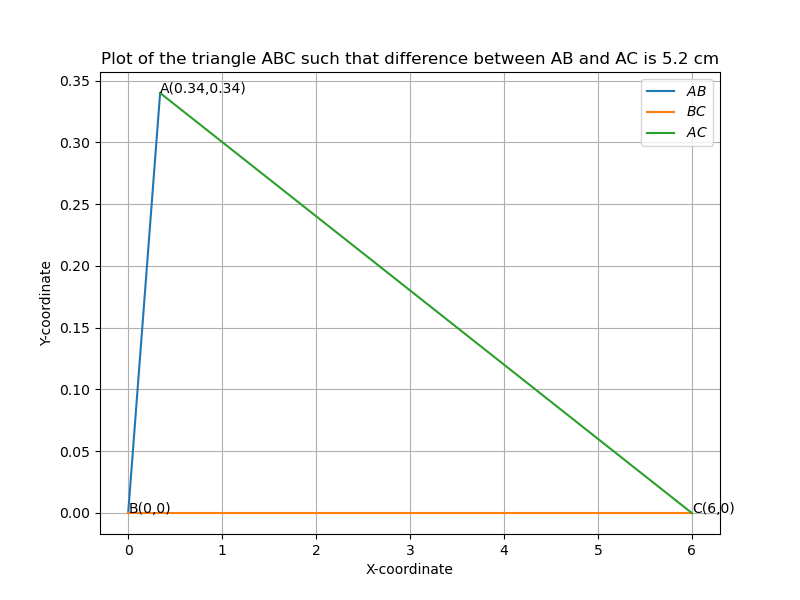
\includegraphics[scale=0.5]{figs/plot1.png}
	\label{Fig}
\end{figure}
\begin{figure}[h]
	\centering
	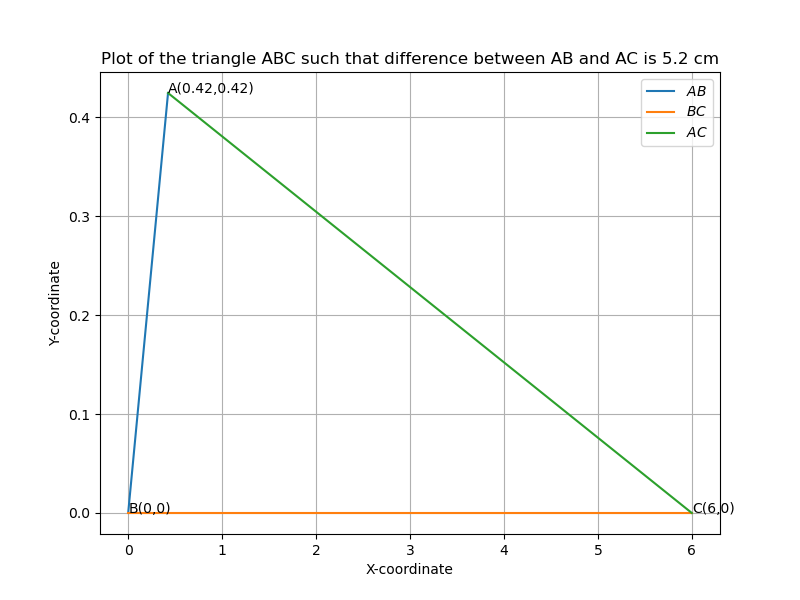
\includegraphics[scale=0.5]{figs/plot2.png}
	\label{Fig}
\end{figure}
\begin{figure}[h]
	\centering
	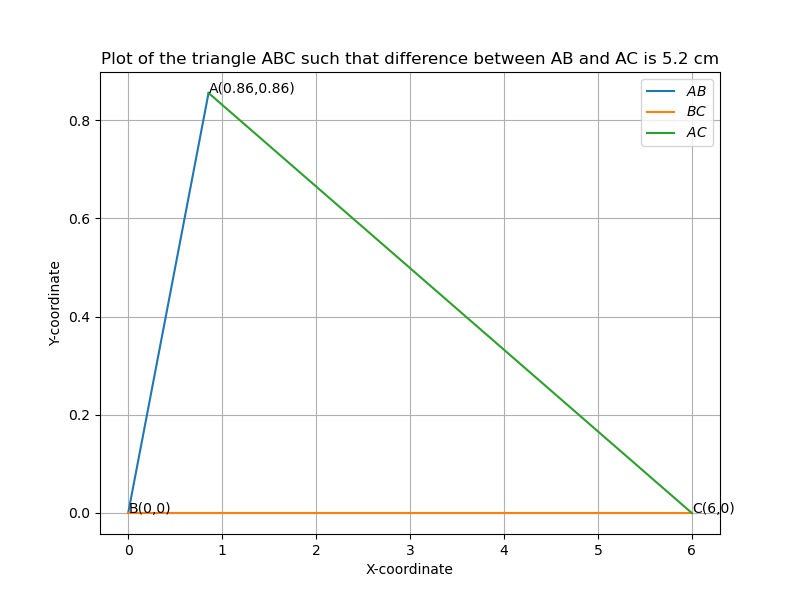
\includegraphics[scale=0.5]{figs/plot3.png}
	\label{Fig}
\end{figure}
\end{document}
